
\documentclass{article}
\usepackage[utf8]{inputenc}
\usepackage[spanish]{babel}
\usepackage{graphicx}
\usepackage{geometry}
\usepackage{enumerate}
\usepackage{titlesec}
\usepackage{float}

\geometry{letterpaper, margin = 1.5cm}

%Datos de la Portada
\title{Herrramientas Computacionales \\ Practica 1}
\author{Medina Martinez Jonathan Jason \\ 2023640061}
\date{22 de febrero de 2023}

\begin{document} %Inicio del Documento

\fontsize{12}{14}\selectfont

\begin{figure}[t] %Logos Portada


\includegraphics[width=2.5 cm]{Logo1.jpeg}
\hfill

\includegraphics[width=3 cm]{Logo2.png}

\end{figure}

\maketitle %Titulo Portada
\newpage

\tableofcontents %Indice
\newpage

\section{Objetivo}

Aplicar operaciones y visualizar los resultados en las ventanas de trabajo.

\section{Introducción}

\subsection{Ventanas de trabajo}
Las partes principales de la interfaz de matlab son las siguientes:

\begin{figure}[H]
    \centering
    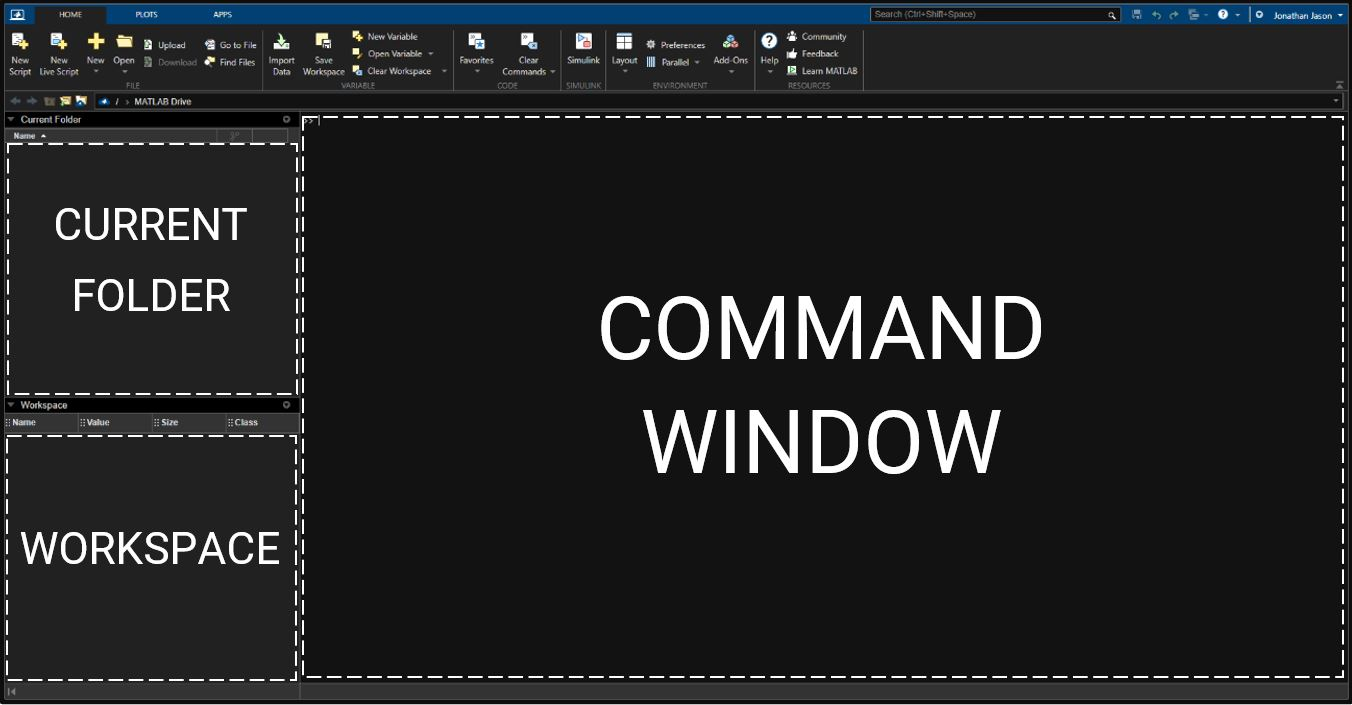
\includegraphics[width=18cm]{partes.jpg}
    \label{fig:my_label}
\end{figure}

\subsubsection{Current Folder}

Current folder o Carpeta actual muestra la carpeta que se esta utilizando en ese momento.

\subsubsection{Workspace}

Aqui se muestran las variables y los valores que se an guardado en dichas variables

\subsubsection{Command Window}

Aqui se muestran todos lo comandos utilizados anteriormente que no se allan borrado ademas de todos los nuevos comandos que se realizen.

\newpage

\section{Desarrollo}

\subsubsection{Cree las carpetas C:/Matlab/P21/ y cambie su Current Folder a dicha carpeta}

\begin{enumerate}
    \item Usamos el comando mkdir para generar la carpeta.
    \item Utilizamos  el comando cd para cambiar el current folder a la nueva carpeta.
\end{enumerate}

\begin{figure}[H]
    \centering
    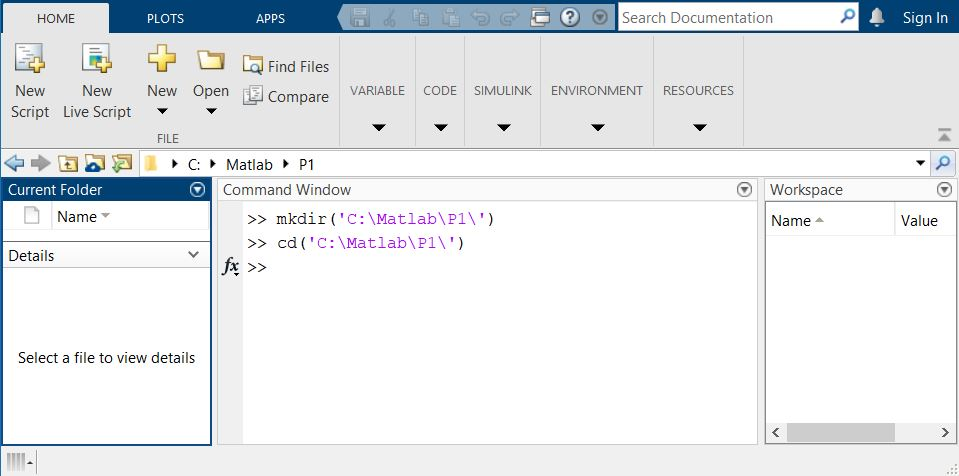
\includegraphics[width=18cm]{img1.jpg}
\end{figure}

\subsubsection{Escriba la expresion 2 + 3 ∗ 4 en la ventana Command Window y presione ENTER, ¿Que ocurre en la ventana Workspace?}

\begin{figure}[H]
    \centering
    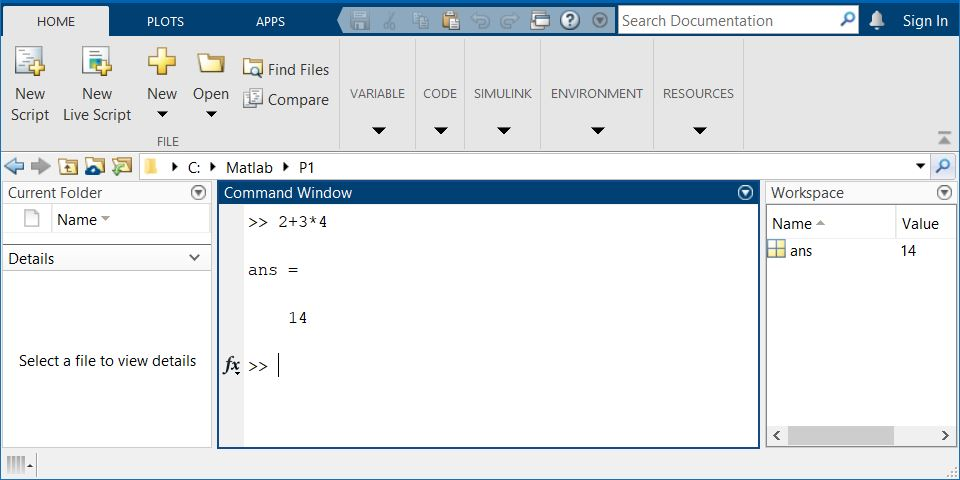
\includegraphics[width=18cm]{img2.jpg}
\end{figure}

\subsubsection{¿Que representa la variable ans que se observa en Workspace?}

La variable ans se utiliza para almacenar el resultado de la última operación realizada que no se ha almacenado en otra variable.

\subsubsection{Limpie su Workspace utilizando el comando clear en la ventana Command Window}

El comando \textbf{clear} limpia las variables almacenadas en memoria.

\begin{figure}[H]
    \centering
    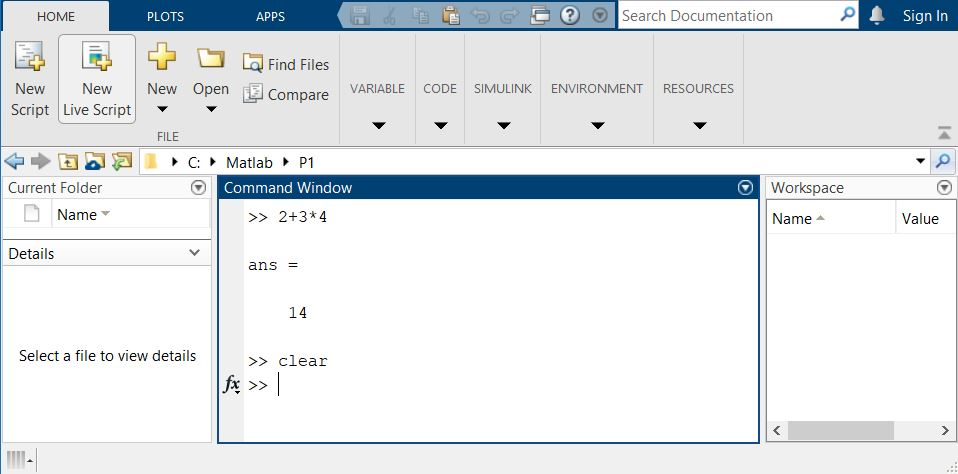
\includegraphics[width=18cm]{img3.jpg}
\end{figure}

\subsubsection{Limpie su Command Window utilizando un comando}

El comando \textbf{clc} limpia el command window.

\begin{figure}[H]
    \centering
    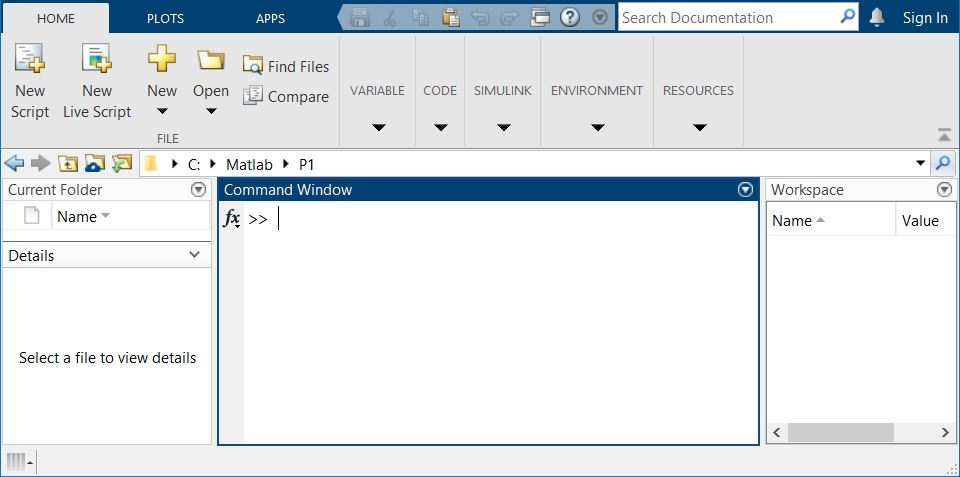
\includegraphics[width=18cm]{img4.jpg}
\end{figure}

\subsubsection{¿Para que sirve la ventana Command History? y ¿Como puede visualizarse?}

Al presionar la fleca hacia arriba se despliega la ventana Command History.

\begin{figure}[H]
    \centering
    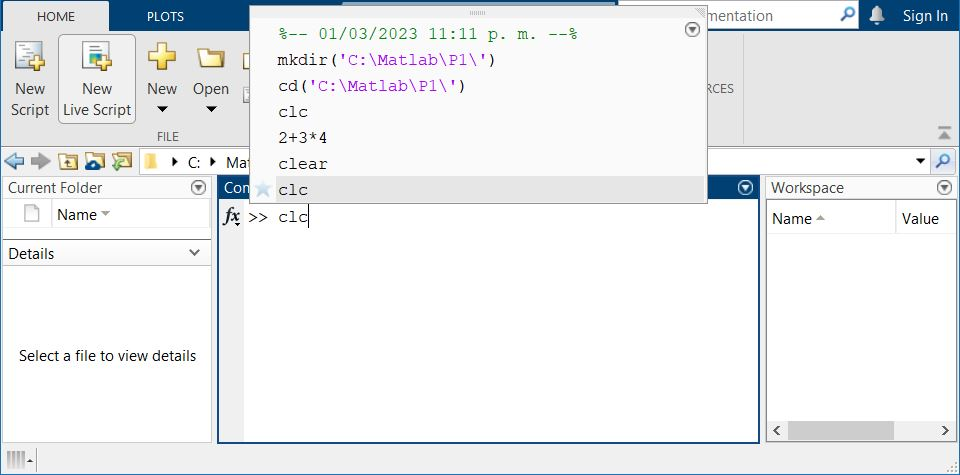
\includegraphics[width=18cm]{img5.jpg}
\end{figure}

\subsection{Operaciones}

\subsubsection{Dada la siguiente lista de nombres de variables, determine cuales son validas y cuales no lo son utilizando el comando isvarname.}

El comando \textbf{isvarname} nos permite saber si el nombre de una variable se puede usar o si este no lo permite, si el nombre es usable nos dara como respuesta 1, sin embargo, si este no es usable nos dara como respuesta 0.

\begin{enumerate}[a)]
    \item test
        \begin{figure}[H]
        \centering
        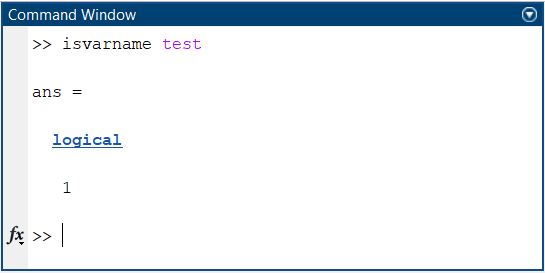
\includegraphics[height=4cm]{img6a.jpg}
        \end{figure}
    \item Test
        \begin{figure}[H]
        \centering
        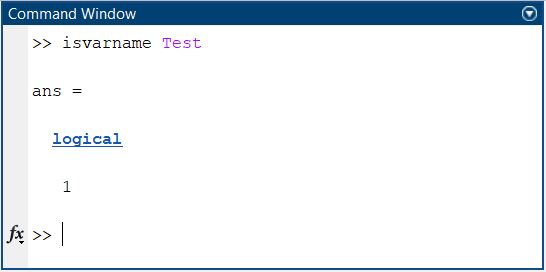
\includegraphics[height=4cm]{img6b.jpg}
        \end{figure}
    \item if
        \begin{figure}[H]
        \centering
        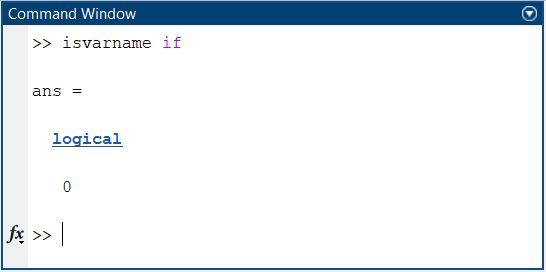
\includegraphics[height=4.8cm]{img6c.jpg}
        \end{figure}
    \item mi-libro
        \begin{figure}[H]
        \centering
        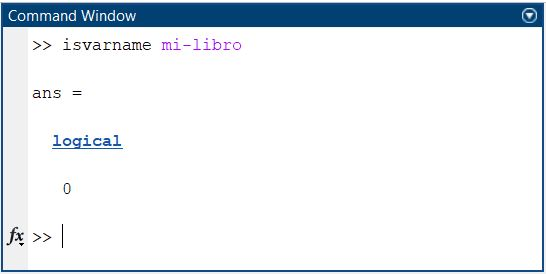
\includegraphics[height=4.8cm]{img6d.jpg}
        \end{figure}
    \item mi\_libro
        \begin{figure}[H]
        \centering
        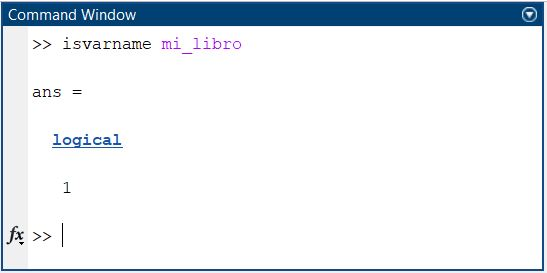
\includegraphics[height=4.8cm]{img6e.jpg}
        \end{figure}
    \item Esteesunnombremuylargoperoinclusoasisepermite?
        \begin{figure}[H]
        \centering
        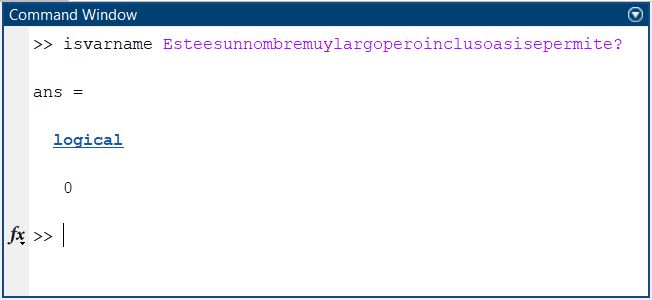
\includegraphics[height=4.8cm]{img6f.jpg}
        \end{figure}
    \item 1ergrupo
        \begin{figure}[H]
        \centering
        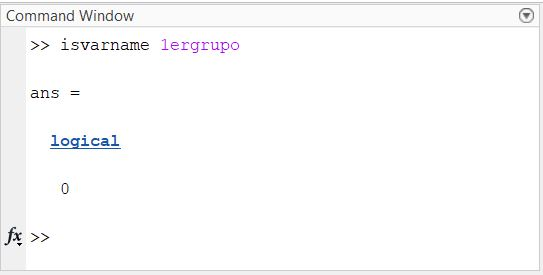
\includegraphics[height=4.8cm]{img6g.jpg}
        \end{figure}
    \item grupo\_uno
        \begin{figure}[H]
        \centering
        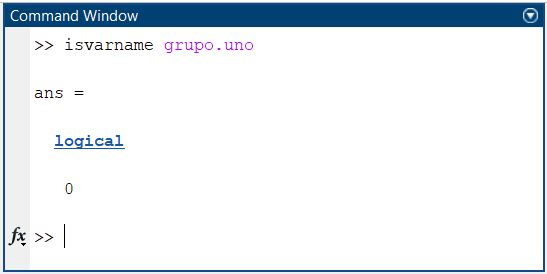
\includegraphics[height=4.8cm]{img6h.jpg}
        \end{figure}
    \item zzaAbc
        \begin{figure}[H]
        \centering
        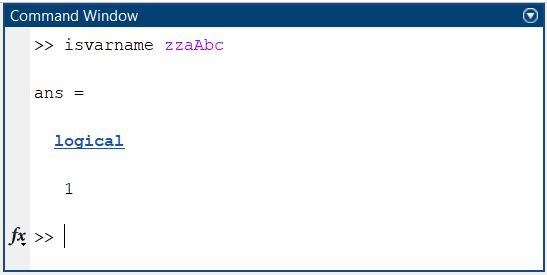
\includegraphics[height=4.8cm]{img6i.jpg}
        \end{figure}
    \item z34wAwy?12\#
        \begin{figure}[H]
        \centering
        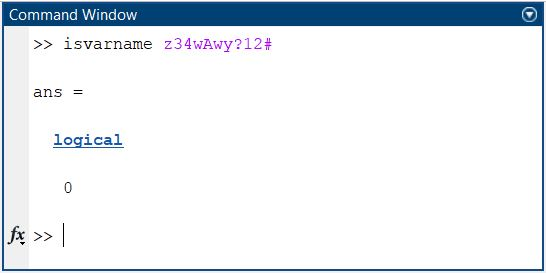
\includegraphics[height=4.8cm]{img6j.jpg}
        \end{figure}
    \item sin
        \begin{figure}[H]
        \centering
        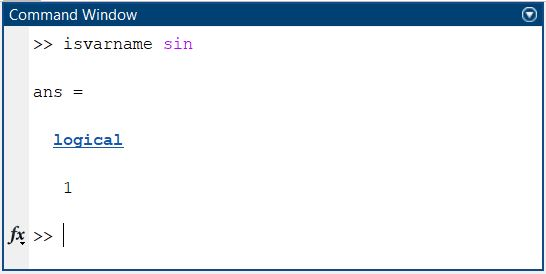
\includegraphics[height=4.8cm]{img6k.jpg}
        \end{figure}
    \item log
        \begin{figure}[H]
        \centering
        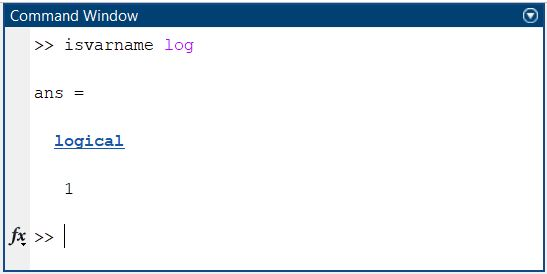
\includegraphics[height=4.8cm]{img6l.jpg}
        \end{figure}
    \item fred
        \begin{figure}[H]
        \centering
        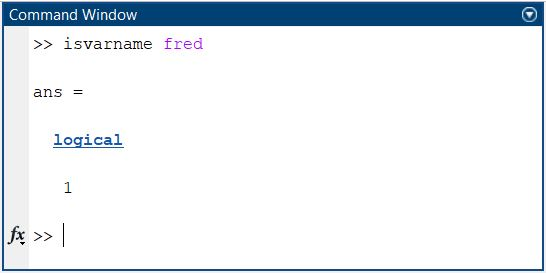
\includegraphics[height=4.8cm]{img6m.jpg}
        \end{figure}
    \item fred!
        \begin{figure}[H]
        \centering
        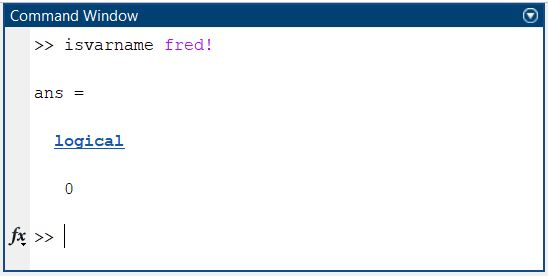
\includegraphics[height=4.8cm]{img6n.jpg}
        \end{figure}
    \item book\_1
        \begin{figure}[H]
        \centering
        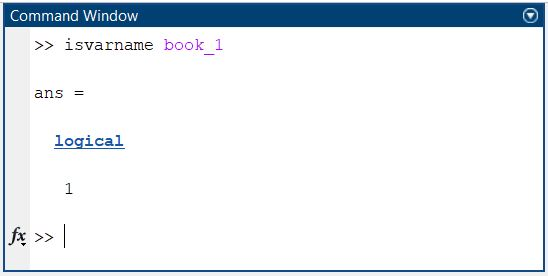
\includegraphics[height=4.8cm]{img6x.jpg}
        \end{figure}
    \item book-1
        \begin{figure}[H]
        \centering
        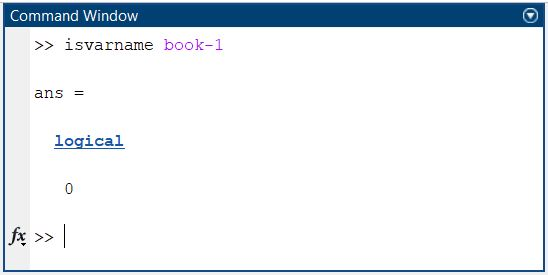
\includegraphics[height=4.8cm]{img6o.jpg}
        \end{figure}
    \item 2ndplace
        \begin{figure}[H]
        \centering
        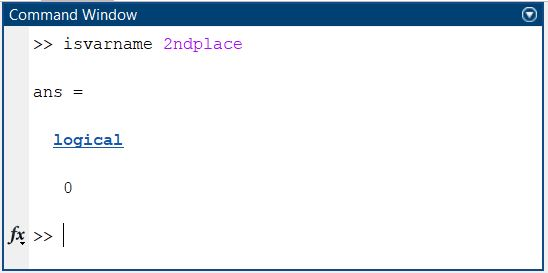
\includegraphics[height=4.8cm]{img6p.jpg}
        \end{figure}
    \item Second\_Place
        \begin{figure}[H]
        \centering
        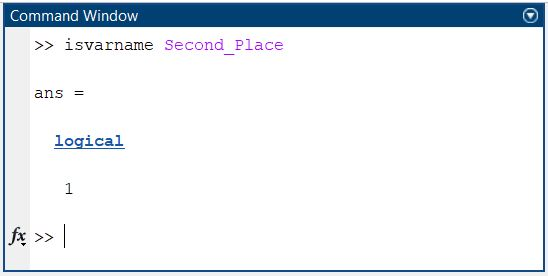
\includegraphics[height=4.8cm]{img6q.jpg}
        \end{figure}
    \item \#1
        \begin{figure}[H]
        \centering
        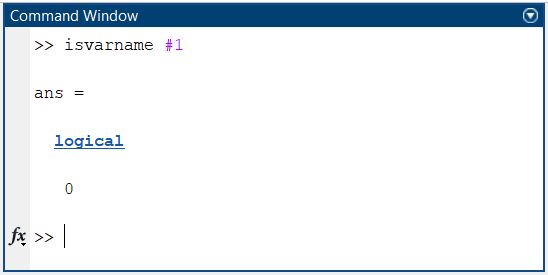
\includegraphics[height=4.8cm]{img6r.jpg}
        \end{figure}
    \item No\_1
        \begin{figure}[H]
        \centering
        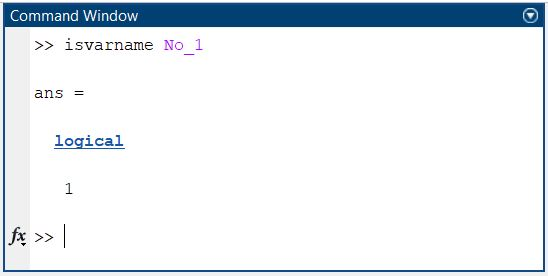
\includegraphics[height=4.8cm]{img6s.jpg}
        \end{figure}
    \item vel\_5
        \begin{figure}[H]
        \centering
        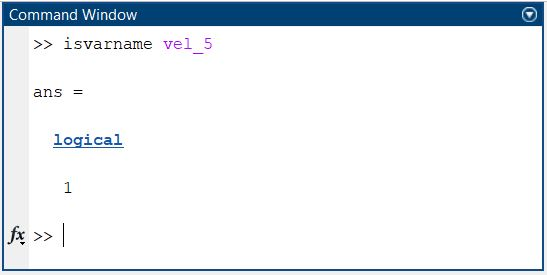
\includegraphics[height=4.8cm]{img6t.jpg}
        \end{figure}
    \item vel.5
        \begin{figure}[H]
        \centering
        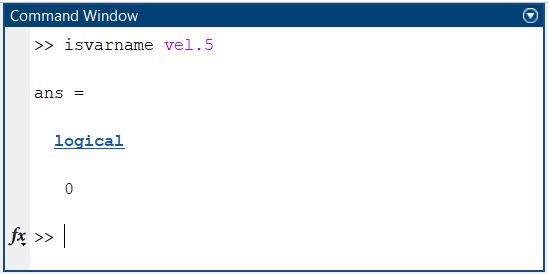
\includegraphics[height=4.8cm]{img6u.jpg}
        \end{figure}
    \item tan
        \begin{figure}[H]
        \centering
        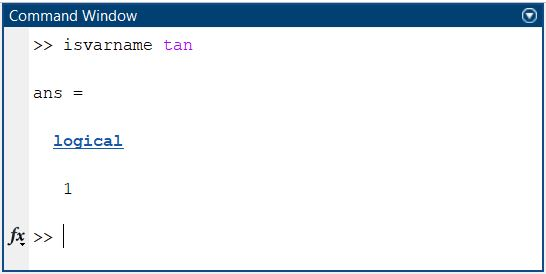
\includegraphics[height=4.8cm]{img6v.jpg}
        \end{figure}
    \item while
        \begin{figure}[H]
        \centering
        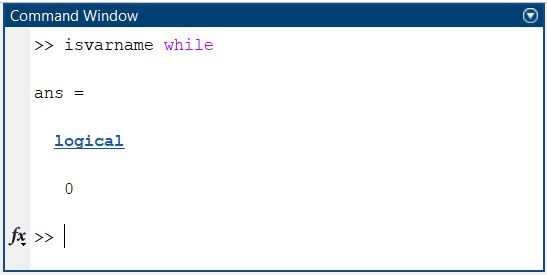
\includegraphics[height=4.8cm]{img6w.jpg}
        \end{figure}
\end{enumerate}

\subsubsection{De los nombres de variables no validos de la lista anterior, explique el motivo por el cual no son validos.}

Los nombres de esas variables no son validos por las siguientes reglas:

\begin{itemize}
    \item Los nombres de las variables no pueden comenzar con números
    \item Los nombre de variables pueden tener solo letras, números y \_
    \item Los nombres de variables tienen un máximo de 63 (namelengthmax)
\end{itemize}
\newpage
\subsubsection{Utilizando la ventana Command Window de MATLAB, resuelva las siguientes operaciones. Para cada operacion, debera mostrar los resultados en los formatos long, short y rat.}

\begin{enumerate}[a)]
    \item $$a = \frac{25.7 * 62 - 7^{3.1}}{45 + 5^2}$$
        \begin{figure}[H]
        \centering
        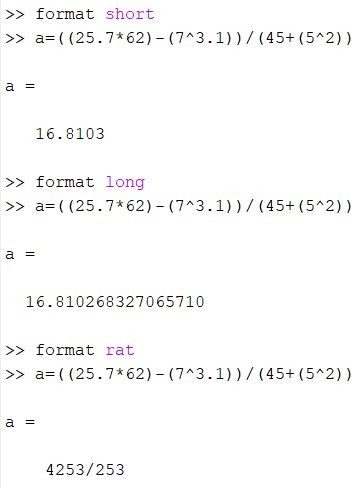
\includegraphics[height=9cm]{img7a.jpg}
        \end{figure}
    \item $$b = \frac{4}{7} * 7 * 6^3 + \frac{3^6}{9^3 - 652}$$
        \begin{figure}[H]
        \centering
        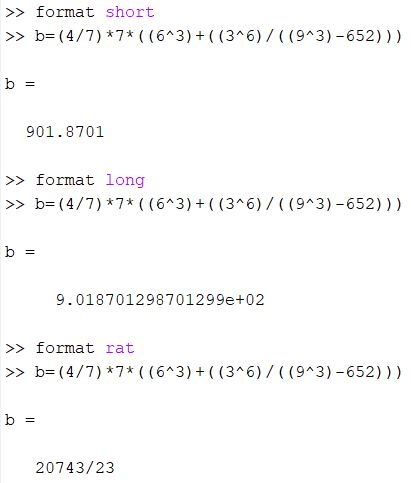
\includegraphics[height=9cm]{img7b.jpg}
        \end{figure}
    \item $$c = \left(2+7\right)^4 + \frac{27.3^{2/3}}{2} + \frac{55^{3/4}}{3}$$
        \begin{figure}[H]
        \centering
        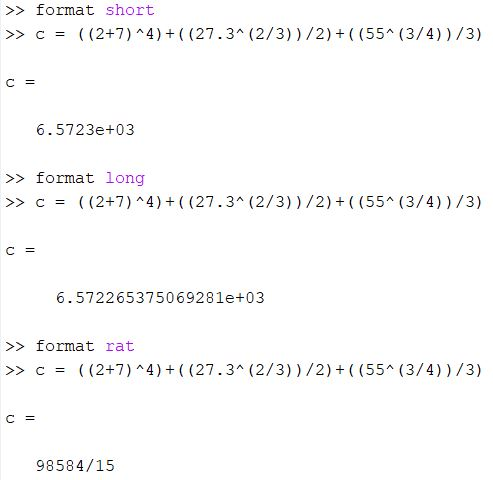
\includegraphics[height=10cm]{img7c.jpg}
        \end{figure}
    \item $$d = 2.5^3 + 7.3^3 + \frac{273^3}{5} + 55^\frac{1}{2}$$
        \begin{figure}[H]
        \centering
        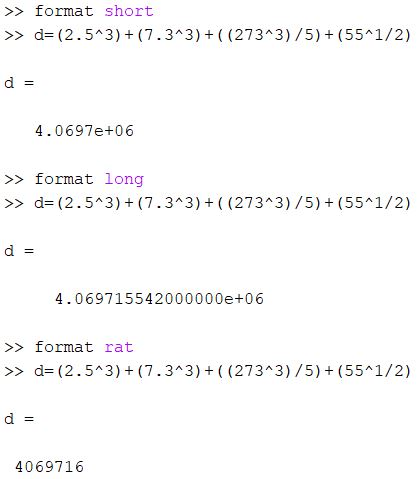
\includegraphics[height=10cm]{img7d.jpg}
        \end{figure}
    \item $$e = \frac{5 + 6\left(\frac{7}{3}\right) - 2^2}{\left(\frac{4}{3}\right)\left(\frac{1}{3\left(6^2\right)}\right)}$$
        \begin{figure}[H]
        \centering
        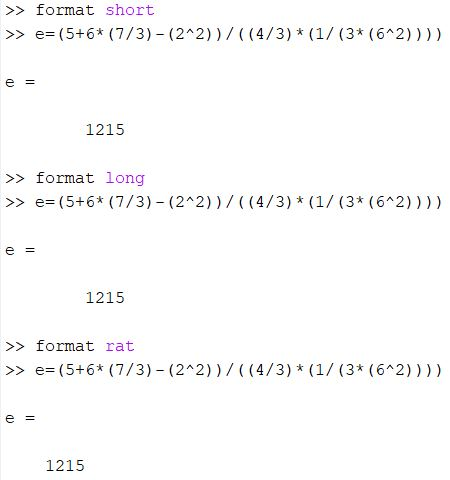
\includegraphics[height=10cm]{img7e.jpg}
        \end{figure}
    \item $$f = \frac{6}{12} + 7 * \sqrt[3]{4+6^2}$$
        \begin{figure}[H]
        \centering
        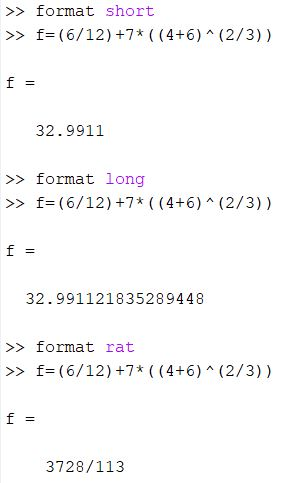
\includegraphics[height=10cm]{img7f.jpg}
        \end{figure}
    \item Calcule el  ́area de un circulo de radio 15. Guarde el resultado en la variable g.
        \begin{figure}[H]
        \centering
        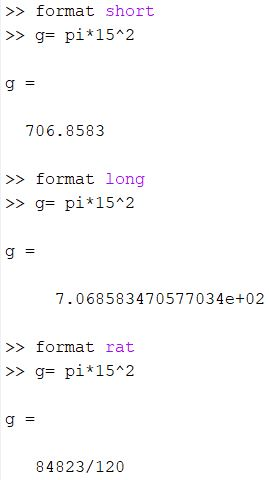
\includegraphics[height=10cm]{img7g.jpg}
        \end{figure}
    \item Calcule el  ́area superficial de una esfera de radio 35. Guarde su resultado en la variable h.
        \begin{figure}[H]
        \centering
        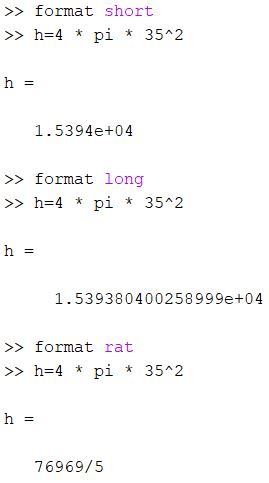
\includegraphics[height=10cm]{img7h.jpg}
        \end{figure}
    \newpage
    \item Calcule el volumen de una esfera de radio 45. Guarde su resultado en la variable i.
        \begin{figure}[H]
        \centering
        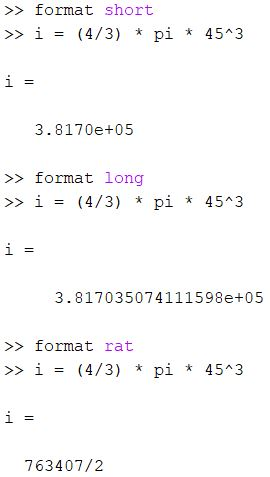
\includegraphics[height=10cm]{img7i.jpg}
        \end{figure}
\end{enumerate}

\section{Conclusiones}

Matlab nos permite relizar operaciones desde las mas basicas a muy avanzadas ademas de almacenar gran variedad de variables las cuales nos permiten realizar funciones y programas sin la nececidad de estar repitiendo datos o formulas.

\end{document}